\chapter{Oscillations}
We just finished up a chapter about circular motion, where objects move around in a circle at either constant (uniform/harmonic) or changing (non-uniform) speeds. 

In this chapter, we will study oscillatory motion, which is a type of motion where an object moves back and forth around an equilibrium point. Oscillations are common in many physical systems, such as springs, pendulums, and even electrical circuits. Oscillations are important not only because they appear everywhere in physical systems, but also because they provide a connection between simple motion and more complex behaviors. Small oscillations often behave in a very predictable way and can be described using \emph{simple harmonic motion} (SHM), which is governed by restoring forces proportional to displacement.

We will also give an introduction to \emph{differential equations} used to model oscillatory systems, often found in engineering and physics. 

\section{Sine and Cosine Graphs [Review]}
Let's recall the two pillars of trigonometry and, consequently, simple harmonic motion: Sine and Cosine. Recall that these two functions are periodic, meaning they repeat their values in regular intervals or periods. The sine and cosine functions have a period of \(2\pi\) radians or 360$^\circ$, repeating their values every \(2\pi\) radians.

As discussed in the circular motion chapter, the sine function represents the y-coordinate of a point on the unit circle as it moves around the circle, while the cosine function represents the x-coordinate. This is the fundemental behavior of the unit circle, where a point moves around the circle at a constant angular speed \(\omega\). The position of the point at any time \(t\) can be described using the following parametric equations:
$$x(t) = \cos(\omega t), \qquad y(t) = \sin(\omega t)$$

The general forms of the sine and cosine functions can be expressed as:
$$x(t) = A\cos(\omega t + \phi), \qquad y(t) = A\sin(\omega t + \phi)$$

where:
\begin{itemize}
    \item \(A\) is the amplitude, representing the maximum displacement from the equilibrium position.
    \item \(\omega\) is the angular speed, which determines how quickly the oscillations occur.
    \item \(\phi\) is the phase shift, which determines the initial position of the oscillation at \(t = 0\).
\end{itemize}

Recall that the derivatives of these functions are also periodic, a key property that is useful for analyzing oscillatory motion:
$$\frac{d}{dt}\cos(\omega t) = -\omega \sin(\omega t)$$
$$\frac{d}{dt}\sin(\omega t) = \omega \cos(\omega t)$$
$$\frac{d^2}{dt^2}\cos(\omega t) = -\omega^2 \cos(\omega t)$$

In the motion we will talk about,
\begin{itemize}
    \item $x(t)$ will be our position function
    \item $v(t)$ describes our velocity function, which can be the first derivative of our position
    \item $a(t)$ is our acceleration function, derived from $v(t)$
\end{itemize}
We notice that the second derivative produces a negative multiple of the original function. This can be simplified in terms of acceleration and position functions: $a(t) = -\omega^2 x(t)$.


\section{Simple Harmonic Motion}
\index{SHM|see{simple harmonic motion}}
\index{simple harmonic motion}
Simple Harmonic Motion will reference many definitions we have seen before and will continue to see in this chapter. Here are some key terms to know:
\begin{description}
    \item[Cycle] A single complete execution of a periodically repeated motion. Another way to think about it is a particle, block, or object making a \emph{round-trip}.
    \item[Period] The time it takes to complete one cycle of motion. An identity that comes up often is $T= \frac{2\pi}{\omega}$.
    \item[Frequency] The number of cycles completed per unit time. It is the reciprocal of the period, represented as $\mathbf{Hz}$.\footnote{One $\mathbf{Hz}$ is equal to one cycle per second. For example, a frequency of 5 Hz means that 5 cycles are completed in one second. On a monitor, a refresh rate of 60 Hz means the screen updates 60 times per second. Higher refresh rates can lead to smoother motion perception.}
    \item[Equilibrium] The position at which the ``default'' position of an oscillating object is located. In terms of mechanics, this is the position where all the forces acting on the object are balanced or zero.
    \item[Restoring Force] The force that acts to bring an oscillating object back to its equilibrium position. It is typically proportional to the displacement from equilibrium and acts in the opposite direction.
    \item[Angular Speed] The rate at which an object moves around a circle, measured in radians per second. 
\end{description}


So far, we have discussed oscillatory motion in general terms. Now, let's focus on a specific type of oscillatory motion known as Simple Harmonic Motion (SHM). SHM is characterized by the following properties:
\begin{itemize}
    \item The motion occurs around an equilibrium position.
    \item The \emph{restoring force} is directly proportional to the displacement from the equilibrium position and acts in the opposite direction.\index{restoring force}
    \item The motion is sinusoidal in nature, meaning it can be described using sine or cosine functions.
    \item The period and frequency of the motion are constant, regardless of the amplitude.
    \item The acceleration always points toward equilibrium and increases in size as the displacement grows.

\end{itemize}
So the motion continously repeats itself in a regular pattern. It speeds up near equilibrium, and slows down to a stop at maximum displacement.
Examples of these systems are
\begin{itemize}
    \item A mass attached to a spring, either vertically or horizontally
    \item A simple pendulum 
    \item Vibrations of a tuning fork or guitar string
\end{itemize}

We saw in our pendulums chapter how the system has both centripetal acceleration and acceleration due to gravity, causing oscillations back and forth with changing speed.
\index{simple harmonic motion!energy in}
Like all mechanical systems, an SHM system has both kinetic and potential energy. For general simple harmonic motion systems, we can describe its energy as follows:
\begin{itemize}
    \item The total mechanical energy \(E\) of the system is the sum of its kinetic energy \(K\) and potential energy \(U\):
    $$E = K + U$$
    \item The kinetic energy \(K\), system dependent, is highest when the object passes through the equilibrium position.
    \item The potential energy \(U\) depends on the specific system, such as spring potential energy or gravitational potential energy, but is highest at the maximum displacement from equilibrium.
\end{itemize}

\section{Springs}
Let's talk about springs! Springs are mechanical devices, usually made out of some rigid metal material,  that store and release energy through deformation. When a spring is stretched or compressed from its equilibrium position, it exerts a restoring force that tries to bring it back to its original shape. The most common type of spring is a coil spring, which consists of a linear wire would into a helical shape. \index{springs}

\subsection{Hooke's Law}
In 1676, physicist Robert Hooke formulated a principle that describes the behavior of springs, now known as Hooke's Law. Hooke's Law states that the force exerted by an ideal spring is directly proportional to the displacement from its equilibrium position. 

Mathematically, Hooke's Law can be expressed as:\index{hooke's law}
$$F_s = -kx$$
where:
\begin{itemize}
    \item \(F_s\) is the restoring force exerted by the spring (in newtons, N)
    \item \(k\) is the spring constant (in newtons per meter, N/m), which measures the stiffness of the spring. It is spring-specific
    \item \(x\) is the displacement from the equilibrium position (in meters, m)
    \item The negative sign represents the fact that the force attempts to bring the spring back to its equilibrium position.
\end{itemize}


Since we know that force is related to mass and acceleration through Newton's Second Law, we can combine Hooke's Law with Newton's Second Law to analyze the motion of a mass attached to a spring. See Figure~\ref{fig:ms1} for a diagram of a mass-spring system.
\begin{align}
F_s &= ma = -kx \\
ma &= -kx
\end{align}

\begin{figure}[H]
    \centering


    % Gradient Info
    
    \tikzset {_tglifnpyf/.code = {\pgfsetadditionalshadetransform{ \pgftransformshift{\pgfpoint{0 bp } { 0 bp }  }  \pgftransformrotate{0 }  \pgftransformscale{2 }  }}}
    \pgfdeclarehorizontalshading{_qrc0bgeyq}{150bp}{rgb(0bp)=(0.65,0.81,0.87);
    rgb(37.5bp)=(0.65,0.81,0.87);
    rgb(62.5bp)=(0.14,0.33,0.54);
    rgb(100bp)=(0.14,0.33,0.54)}
    \tikzset{every picture/.style={line width=0.75pt}} %set default line width to 0.75pt        

    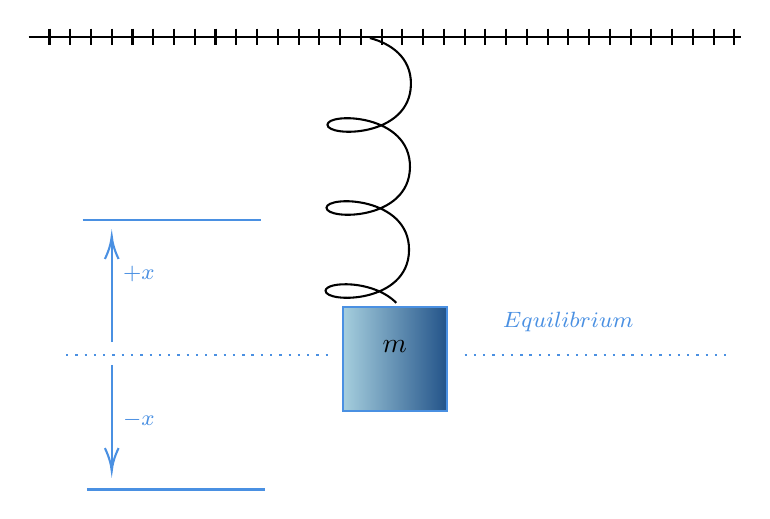
\begin{tikzpicture}[x=0.75pt,y=0.75pt,yscale=-1,xscale=1]
    %uncomment if require: \path (0,300); %set diagram left start at 0, and has height of 300

    %Straight Lines [id:da975132206266746] 
    \draw    (180,42) -- (523,42) (190,38) -- (190,46)(200,38) -- (200,46)(210,38) -- (210,46)(220,38) -- (220,46)(230,38) -- (230,46)(240,38) -- (240,46)(250,38) -- (250,46)(260,38) -- (260,46)(270,38) -- (270,46)(280,38) -- (280,46)(290,38) -- (290,46)(300,38) -- (300,46)(310,38) -- (310,46)(320,38) -- (320,46)(330,38) -- (330,46)(340,38) -- (340,46)(350,38) -- (350,46)(360,38) -- (360,46)(370,38) -- (370,46)(380,38) -- (380,46)(390,38) -- (390,46)(400,38) -- (400,46)(410,38) -- (410,46)(420,38) -- (420,46)(430,38) -- (430,46)(440,38) -- (440,46)(450,38) -- (450,46)(460,38) -- (460,46)(470,38) -- (470,46)(480,38) -- (480,46)(490,38) -- (490,46)(500,38) -- (500,46)(510,38) -- (510,46)(520,38) -- (520,46) ;
    %Shape: Spring [id:dp9925670570214391] 
    \draw   (344.4,42.5) .. controls (354.37,45.12) and (364.29,51.73) .. (364.15,64.73) .. controls (363.85,90.73) and (323.85,90.27) .. (323.92,84.27) .. controls (323.99,78.27) and (363.99,78.73) .. (363.69,104.73) .. controls (363.4,130.72) and (323.4,130.27) .. (323.47,124.27) .. controls (323.54,118.27) and (363.53,118.72) .. (363.24,144.72) .. controls (362.94,170.72) and (322.95,170.27) .. (323.01,164.27) .. controls (323.07,159.71) and (346.12,158.88) .. (357.1,170.1) ;
    %Shape: Square [id:dp37727267362580574] 
    \path  [shading=_qrc0bgeyq,_tglifnpyf] (331.33,172) -- (381.33,172) -- (381.33,222) -- (331.33,222) -- cycle ; % for fading 
    \draw  [color={rgb, 255:red, 74; green, 144; blue, 226 }  ,draw opacity=1 ] (331.33,172) -- (381.33,172) -- (381.33,222) -- (331.33,222) -- cycle ; % for border 

    %Straight Lines [id:da21597477585760394] 
    \draw [color={rgb, 255:red, 74; green, 144; blue, 226 }  ,draw opacity=1 ] [dash pattern={on 0.84pt off 2.51pt}]  (390,195) -- (519,195) ;
    %Straight Lines [id:da8878939995838687] 
    \draw [color={rgb, 255:red, 74; green, 144; blue, 226 }  ,draw opacity=1 ] [dash pattern={on 0.84pt off 2.51pt}]  (198,195) -- (327,195) ;
    %Straight Lines [id:da6678986285537133] 
    \draw [color={rgb, 255:red, 74; green, 144; blue, 226 }  ,draw opacity=1 ]   (220,189) -- (220,140) ;
    \draw [shift={(220,138)}, rotate = 90] [color={rgb, 255:red, 74; green, 144; blue, 226 }  ,draw opacity=1 ][line width=0.75]    (10.93,-3.29) .. controls (6.95,-1.4) and (3.31,-0.3) .. (0,0) .. controls (3.31,0.3) and (6.95,1.4) .. (10.93,3.29)   ;
    %Straight Lines [id:da9876215141273116] 
    \draw [color={rgb, 255:red, 74; green, 144; blue, 226 }  ,draw opacity=1 ]   (220,200) -- (220,249) ;
    \draw [shift={(220,251)}, rotate = 270] [color={rgb, 255:red, 74; green, 144; blue, 226 }  ,draw opacity=1 ][line width=0.75]    (10.93,-3.29) .. controls (6.95,-1.4) and (3.31,-0.3) .. (0,0) .. controls (3.31,0.3) and (6.95,1.4) .. (10.93,3.29)   ;
    %Straight Lines [id:da02119123754763541] 
    \draw [color={rgb, 255:red, 74; green, 144; blue, 226 }  ,draw opacity=1 ]   (206,130) -- (292,130) ;
    %Straight Lines [id:da687106474047876] 
    \draw [color={rgb, 255:red, 74; green, 144; blue, 226 }  ,draw opacity=1 ]   (208,260) -- (294,260) ;

    % Text Node
    \draw (349,187) node [anchor=north west][inner sep=0.75pt]   [align=left] {$\displaystyle m$};
    % Text Node
    \draw (407,173) node [anchor=north west][inner sep=0.75pt]  [font=\footnotesize,color={rgb, 255:red, 74; green, 144; blue, 226 }  ,opacity=1 ] [align=left] {$\displaystyle Equilibrium$};
    % Text Node
    \draw (224,151) node [anchor=north west][inner sep=0.75pt]  [font=\footnotesize,color={rgb, 255:red, 74; green, 144; blue, 226 }  ,opacity=1 ] [align=left] {$\displaystyle +x$};
    % Text Node
    \draw (224,221) node [anchor=north west][inner sep=0.75pt]  [font=\footnotesize,color={rgb, 255:red, 74; green, 144; blue, 226 }  ,opacity=1 ] [align=left] {$\displaystyle -x$};


    \end{tikzpicture}
    \caption{A diagram showing a block of mass $m$ displaced $+x$ and $-x$ from equilibrium.}
    \label{fig:ms1}
\end{figure}

But since above we found a relation between acceleration and position, we can write:

\begin{align}
m \frac{d^2 x}{dt^2} &= -kx \\
\frac{d^2 x}{dt^2} + \frac{k}{m} x &= 0 \label{eq:linearequation}
\end{align}

We can see that this equation describes simple harmonic motion, where the acceleration is proportional to the negative of the displacement. In this form, we can identify the angular speed \(\omega\) of the oscillation as:
$$\omega = \sqrt{\frac{k}{m}}$$ as the term in front of the $x$ in equation~\eqref{eq:linearequation} is $\omega^2$. Thus, we can further define the period as $$T = 2\pi \sqrt{\frac{m}{k}}$$ and the frequency as $$f = \frac{1}{2\pi} \sqrt{\frac{k}{m}}$$

In a later section of this chapter, we will solve this differential equation to find the position function \(x(t)\) of general mass-spring systems.

\begin{Exercise}[label={ex:springmassfreq}, title={Mass-Spring Frequency Change}]
    A block is attached to a spring and set into oscillatory motion, and its frequency is measured. If this block were removed and replace with a block of $1/2$ the mass, how would the frequency of oscillations compare to the original frequency?
    \begin{enumerate}[]
        \item The frequency would be halved.
        \item The frequency would remain the same.
        \item The frequency would increase by a factor of $\sqrt{2}$.
        \item The frequency would decrease by a factor of $\sqrt{2}$.
    \end{enumerate}
\end{Exercise}

\begin{Answer}[ref={ex:springmassfreq}]
    The correct answer is: The frequency would increase by a factor of $\sqrt{2}$.

    The frequency of oscillation for a mass-spring system is given by the formula:
    $$f = \frac{1}{2\pi} \sqrt{\frac{k}{m}}$$
    where \(k\) is the spring constant and \(m\) is the mass attached to the spring.
    Since frequency is inversely proportional to the square root of the mass, if the mass is halved, the new frequency \(f'\) can be calculated as follows:
    \begin{align*}
    f' &= \frac{1}{2\pi} \sqrt{\frac{k}{m/2}} \\
    &= \frac{1}{2\pi} \sqrt{\frac{2k}{m}} \\
    &= \sqrt{2} \cdot \frac{1}{2\pi} \sqrt{\frac{k}{m}} \\
    &= \sqrt{2} \cdot f
    \end{align*}
    Therefore, the frequency increases by a factor of \(\sqrt{2}\) when the
\end{Answer}
\subsection{Spring Potential Energy}
\index{springs!spring potential energy}
Let's recall that Work from a physics standpoint is defined as the transfer of energy through a certain distance via a force. When we alter the length of a spring through either compression or extenson, we are performing work on the spring. This work is stored as potential energy within the spring, which can be released when the spring returns to its equilibrium position.

Let's find an equation for this change in potential energy, which gets stored up in the spring. Recall the two mathematical definitions for work:
\begin{itemize}
    \item Work as the product of force and distance: \(W = F \cdot d\)
    \item Work as the integral of force over a distance: \(W = \int F \, dx\)
\end{itemize}
We need to use the integral definition, since, by our definition of Hooke's Law, the force exerted by a spring varies with displacement, so every tiny bit of distance, or $dx$ is different. For any spring starting at equilibrium (0), and moving to some final position $x_f$, we can write:
\begin{align*}
W &= \int_{x_i}^{x_f} F_x \, dx \\
W_s &= \int_{x_i}^{x_f} F_s \, dx \\
&= \int_{0}^{x_f} -kx \, dx \\
&= \frac{-kx^2}{2} \bigg|_0^{x_f}\\
% &= \frac{-k{x_f}^2}{2} - 0 \\
&= \frac{-k({x_f})^2}{2}  
\end{align*}

This work done on the spring is stored as potential energy, so we can say that the change in potential energy of the spring is equal to the negative of the work done by the spring force:
\begin{equation}
    \Delta U_s = -W_s = \frac{1}{2} k x_f^2
    \label{springpe}
\end{equation}
We can see this graphically in Figure~\ref{fig:springpe}, where the area under the force vs. displacement graph represents the work done on the spring, which is equal to the change in potential energy.

\begin{figure}[H]
    \centering




    \tikzset{every picture/.style={line width=0.75pt}} %set default line width to 0.75pt        

    \begin{tikzpicture}[x=0.75pt,y=0.75pt,yscale=-1,xscale=1]
    %uncomment if require: \path (0,310); %set diagram left start at 0, and has height of 310

    %Shape: Right Triangle [id:dp5200885887106212] 
    \draw  [color={rgb, 255:red, 208; green, 2; blue, 27 }  ,draw opacity=0.77 ][fill={rgb, 255:red, 200; green, 98; blue, 98 }  ,fill opacity=1 ] (124,103) -- (321,202) -- (124,202) -- cycle ;
    %Straight Lines [id:da7631542187045505] 
    \draw [color={rgb, 255:red, 74; green, 144; blue, 226 }  ,draw opacity=1 ]   (112,200) -- (112,100) ;
    \draw [shift={(112,97)}, rotate = 90] [fill={rgb, 255:red, 74; green, 144; blue, 226 }  ,fill opacity=1 ][line width=0.08]  [draw opacity=0] (8.93,-4.29) -- (0,0) -- (8.93,4.29) -- cycle    ;
    \draw [shift={(112,203)}, rotate = 270] [fill={rgb, 255:red, 74; green, 144; blue, 226 }  ,fill opacity=1 ][line width=0.08]  [draw opacity=0] (8.93,-4.29) -- (0,0) -- (8.93,4.29) -- cycle    ;
    %Straight Lines [id:da5146615233869427] 
    \draw [color={rgb, 255:red, 74; green, 144; blue, 226 }  ,draw opacity=1 ]   (339,214) -- (119,214) ;
    \draw [shift={(116,214)}, rotate = 360] [fill={rgb, 255:red, 74; green, 144; blue, 226 }  ,fill opacity=1 ][line width=0.08]  [draw opacity=0] (8.93,-4.29) -- (0,0) -- (8.93,4.29) -- cycle    ;
    \draw [shift={(342,214)}, rotate = 180] [fill={rgb, 255:red, 74; green, 144; blue, 226 }  ,fill opacity=1 ][line width=0.08]  [draw opacity=0] (8.93,-4.29) -- (0,0) -- (8.93,4.29) -- cycle    ;
    %Shape: Axis 2D [id:dp3931603587757937] 
    \draw  (103,202) -- (536.5,202)(321,102.66) -- (321,301) (529.5,197) -- (536.5,202) -- (529.5,207) (316,109.66) -- (321,102.66) -- (326,109.66) (341,197) -- (341,207)(361,197) -- (361,207)(381,197) -- (381,207)(401,197) -- (401,207)(421,197) -- (421,207)(441,197) -- (441,207)(461,197) -- (461,207)(481,197) -- (481,207)(501,197) -- (501,207)(521,197) -- (521,207)(301,197) -- (301,207)(281,197) -- (281,207)(261,197) -- (261,207)(241,197) -- (241,207)(221,197) -- (221,207)(201,197) -- (201,207)(181,197) -- (181,207)(161,197) -- (161,207)(141,197) -- (141,207)(121,197) -- (121,207)(316,182) -- (326,182)(316,162) -- (326,162)(316,142) -- (326,142)(316,122) -- (326,122)(316,222) -- (326,222)(316,242) -- (326,242)(316,262) -- (326,262)(316,282) -- (326,282) ;
    \draw   ;
    %Straight Lines [id:da7205057106226027] 
    \draw [color={rgb, 255:red, 74; green, 144; blue, 226 }  ,draw opacity=1 ]   (76.68,79.35) -- (479.32,281.65) ;
    \draw [shift={(482,283)}, rotate = 206.68] [fill={rgb, 255:red, 74; green, 144; blue, 226 }  ,fill opacity=1 ][line width=0.08]  [draw opacity=0] (8.93,-4.29) -- (0,0) -- (8.93,4.29) -- cycle    ;
    \draw [shift={(74,78)}, rotate = 26.68] [fill={rgb, 255:red, 74; green, 144; blue, 226 }  ,fill opacity=1 ][line width=0.08]  [draw opacity=0] (8.93,-4.29) -- (0,0) -- (8.93,4.29) -- cycle    ;
    %Curve Lines [id:da46276607686239846] 
    \draw [color={rgb, 255:red, 0; green, 0; blue, 0 }  ,draw opacity=1 ][line width=2.25]    (466,99) .. controls (448.18,149) and (336.27,132.34) .. (227.3,186.34) ;
    \draw [shift={(224,188)}, rotate = 333.02] [color={rgb, 255:red, 0; green, 0; blue, 0 }  ,draw opacity=1 ][line width=2.25]    (17.49,-5.26) .. controls (11.12,-2.23) and (5.29,-0.48) .. (0,0) .. controls (5.29,0.48) and (11.12,2.23) .. (17.49,5.26)   ;

    % Text Node
    \draw (201.08,117.29) node [anchor=north west][inner sep=0.75pt]  [rotate=-27.06] [align=left] {\textcolor[rgb]{0.29,0.56,0.89}{$\displaystyle F_{s} =-kx$$ $}};
    % Text Node
    \draw (87.1,140.51) node [anchor=north west][inner sep=0.75pt]  [rotate=-0.62] [align=left] {\textcolor[rgb]{0.29,0.56,0.89}{$\displaystyle kx$}\textcolor[rgb]{0.29,0.56,0.89}{$ $}};
    % Text Node
    \draw (230.97,217.02) node [anchor=north west][inner sep=0.75pt]  [rotate=-0.62] [align=left] {\textcolor[rgb]{0.29,0.56,0.89}{$\displaystyle x$}\textcolor[rgb]{0.29,0.56,0.89}{$ $}};
    % Text Node
    \draw (426,11.4) node [anchor=north west][inner sep=0.75pt]  [color={rgb, 255:red, 74; green, 144; blue, 226 }  ,opacity=1 ]  {$ \begin{array}{l}
    Area\ =\ \frac{1}{2} bh\ =\ \frac{1}{2} kx( x)\\
    \begin{aligned}
    Area= & \frac{1}{2} bh\\
    = & \frac{1}{2}( kx)( x)\\
    = & \frac{1}{2} kx^{2}
    \end{aligned}
    \end{array}$};



    \end{tikzpicture}
    \caption{A graph of force versus displacement for a spring, equal to the work done and change in potential energy.}
    \label{fig:springpe}
\end{figure}


Notice that Equation~\eqref{springpe} is similar in structure to the kinetic energy equation, \(K = \frac{1}{2} mv^2\). This is not a coincidence, as both equations describe forms of energy in mechanical systems, and are derived from linear systems. The big idea is:

When the effort (force) needed increases in direct proportion to what you're trying to change, the energy required ends up depending on the square of that change.

For a spring
\begin{itemize}
    \item[-] the farther you stretch or compress it, the more force it exerts to return to equilibrium (Hooke's Law)
    \item[-] the more energy is stored in the spring (spring potential energy)
\end{itemize}

For kinetic energy
\begin{itemize}
    \item[-] the faster you try to move an object, the more force is needed to accelerate it (Newton's Second Law)
    \item[-] the more energy the object has due to its motion (kinetic energy)
\end{itemize}

\begin{Exercise}[label={ex:springequation}, title={Finding the equation for a mass-spring system}]
    This question is from an AP-style physics review. 
    A block of mass 4 kg on a fricitonless, horizontal table is attached to a spring with spring constant \(k = 400 \, \text{N/m}\) and undergoes simple harmonic oscillations about its equilibrium position and its amplitude $A=6$ cm. If the block is at $x=6$ cm at time $t=0$ and has a velocity of $0$ cm/s at that time, which of the following equations (with $x$ in cm and $t$ in seconds) describes the block's position as a function of time?

    \begin{enumerate}[label=(\Alph*)]
        \item $x(t) = 6 \cos(10t)$
        \item $x(t) = 6 \sin(10t)$
        \item $x(t) = 6 \sin(10t + \frac{1}{2}\pi)$
        \item $x(t) = 6 \sin(10\pi t + \frac{1}{2}\pi)$
        \item $x(t) = 6 \sin(10\pi t - \frac{1}{2}\pi)$
    \end{enumerate}
    
\end{Exercise}
\begin{Answer}[ref={ex:springequation}]
    First, we find the angular frequency \(\omega\) using the formula:
    \[
    w = 2\pi f = \sqrt{\frac{k}{m}} = \sqrt{\frac{400 \, \text{N/m}}{4 \, \text{kg}}} = \sqrt{100} = 10 \, \text{rad/s}
    \]

    Therefore, the general equation for the position of a mass-spring system undergoing simple harmonic motion is:
    \[
    x(t) = A \cos(\omega t + \phi)
    \]
    becomes $x= 6 \sin(10t + \phi)$ since the initial velocity is 0, meaning it starts at maximum displacement. Solving for $\phi$ using the initial condition $x(0) = 6$ cm:
    \[
    6 = 6 \sin(\phi) \implies \sin(\phi) = 1 \implies \phi = \frac{\pi}{2}
    \]  
    So the base equation becomes:
    \[
    x(t) = 6 \sin(10t + \frac{\pi}{2})
    \]  
    Which is option C.
\end{Answer}
\begin{Exercise}[label={ex:shmchars}]
    This question is from an AP-style physics review.

    Which of the following characteristics are true of simple harmonic motion? Select all that apply.
    \begin{enumerate}[label=\Roman*]
        \item The acceleration is constant.
        \item The restoring force is proportional to the displacement from equilibrium.
        \item The frequency is independent of the amplitude.
    \end{enumerate}    
    
    \begin{enumerate}[label=(\alph*)]
        \item II only
        \item I and II only
        \item I and III only
        \item II and III only
    \end{enumerate}
\end{Exercise}

\begin{Answer}[ref={ex:shmchars}]
Assessing statement I: The acceleration in simple harmonic motion is not constant; it varies with displacement. Therefore, statement I is false. (b), (c) cannot be correct. Statement II must be true since it appears in both remaining answer choices. Statement III is also true, as the frequency of simple harmonic motion does not depend on amplitude. Therefore, the correct answer is (d), II and III only.
\end{Answer}

\begin{Exercise}[label={ex:springenergytransfer}, title={Energy Transfer in a Mass-Spring System}]
    A pinball machine uses a spring to launch a ball of mass $0.2$ kg. The spring has a spring constant of $500$ N/m and is compressed by $0.24$ m before release. Assuming energy is conserved and no frictional losses occur, what is the speed of the ball as it leaves the spring?
    
\end{Exercise}
\begin{Answer}[ref={ex:springenergytransfer}]
To find the speed of the ball as it leaves the spring, we can use the principle of conservation of mechanical energy. The net energy in the system remains constant, meaning that the potential energy stored in the compressed spring is converted into the kinetic energy of the ball when it is released.
The potential energy stored in the spring when compressed is given by:
\[U_s = \frac{1}{2} k x^2 = \frac{1}{2} (500) (-0.24)^2 = 14.4 \, \text{J}
\]
The kinetic energy of the ball as it leaves the spring is the same amount, so we set the potential energy equal to the kinetic energy:
\[\frac{1}{2} m v^2 = U_s
\]
Solving for \(v\):
\[v = \sqrt{\frac{2 U_s}{m}} = \sqrt{\frac{2 (14.4)}{0.2}} = \sqrt{144} = 12 \, \text{m/s}\]
The speed of the ball as it leaves the spring is \(12 \, \text{m/s}\).
\end{Answer}

\section{Mass-Spring Systems and Linear Differential Equations}

We have already seen that the motion of a mass attached to a spring can be modeled using differential equations. Here, we will examine this connection more closely.

\subsection{Undamped Simple Harmonic Motion}
Starting from Newton's Second Law and Hooke's Law, we derived the differential equation for simple harmonic motion:
\begin{equation}
m\frac{d^2 x}{dt^2} + kx = 0.
\label{eq:basicshm}
\end{equation}

The term $m\,\frac{d^2 x}{dt^2}$ comes directly from \textit{Newton's Second Law}, representing the net force required to accelerate the mass. The term $kx$ arises from \textit{Hooke's Law}, which states that the spring exerts a restoring force proportional to displacement and directed toward equilibrium.

Equation~\eqref{eq:basicshm} is an example of a \textbf{second-order linear differential equation with constant coefficients without damping}. It describes an ideal mass-spring system with no external influences—one that oscillates forever, undamped and unforced.

The $ma(t)$ term is \textit{Newton's Second Law} part of the equation, while the $kx(t)$ term comes from \textit{Hooke's Law}. This is a second-order linear differential equation with constant coefficients. What if the spring system is being driven by a third force, like friction or damping? We can add an additional force term $F(t)$ to the equation: $F_f(t) = -cv = -cx'$ for forcing function.

\subsection{Introducing Damping}
Real systems are often influenced by additional forces. One common example is a \textbf{damping force}, such as friction or air resistance, which opposes the motion of the mass.

A typical damping force is proportional to the velocity and can be written as
\[
F_d(t) = -c\,\frac{dx}{dt},
\]
where $c$ is the damping coefficient.

Including this force in Newton's Second Law modifies our differential equation. Instead of the undamped equation~\eqref{eq:basicshm}, we obtain:
\begin{align}
m a(t) &= -c\,v(t) - k\,x(t) \label{eq:forcebalance} \\
m\frac{d^2 x}{dt^2} + c\frac{dx}{dt} + kx &= 0 \label{eq:dampedmassspring}
\end{align}


This is still a second-order linear differential equation with constant coefficients, but its solutions behave very differently. Depending on the value of $c$, the system may oscillate with decreasing amplitude, fail to oscillate at all, or return to equilibrium as quickly as possible. 

Finding the roots of the characteristic equation associated with Equation~\eqref{eq:dampedmassspring} allows us to classify the system's behavior into three categories. Recall that the quadratic formula gives us the roots using our coefficients:
$$r = \frac{-c \pm \sqrt{c^2 - 4mk}}{2m}$$

\begin{table}[h!]
\centering
\begin{tabular}{|c|c|c|}
\hline
\textbf{Characteristic Roots} & \textbf{Homogeneous Solution} & \textbf{Damping Type} \\
\hline
$r_1, r_2 \in \mathbb{R}$, both negative 
& $y_h = C_1 e^{r_1 t} + C_2 e^{r_2 t}$ 
& Overdamped \\
\hline
$r$ real, repeated 
& $y_h = (C_1 + C_2 t)e^{rt}$ 
& Critically damped \\
\hline
$r = \alpha \pm i\beta$, $\alpha < 0$ 
& $y_h = e^{\alpha t}\!\left( C_1 \cos(\beta t) + C_2 \sin(\beta t) \right)$ 
& Underdamped \\
\hline
$r = \pm i \beta$ 
& $y_h = C_1 \cos(\beta t) + C_2 \sin(\beta t)$ 
& Simple Harmonic Motion \\
\hline
\end{tabular}
\caption{Classification of solutions to the damped harmonic oscillator based on characteristic roots.}
\end{table}

Without going into too much linear algebra, the function of a mass spring is given by $y(t) = y_h(t) + y_p(t)$, where $y_h$ is the homogeneous solution (the part we solved above by setting the differential equation to 0), and $y_p$ is the particular solution, which depends on any external forcing functions. In this section, we focused on the homogeneous solution. If the equation~\eqref{eq:dampedmassspring} had a forcing function $F(t)$ on the right side, we would need to find a particular solution $y_p$ to account for that.

FIXME solving differential equations given initial conditions
FIXME in book problems about oscillations, which type of damping, etc.


\section{Pendulums}
You may be surprised to know that pendulums act the exact same way as roller coasters from the circular chapter, in terms of forces. But, similar to springs, the oscillate back and forth unless acted upon by a damping force.

A pendulum has an equilibrium position $\theta=0$ such that it is parallel to its gravitational component. A pendulum also has a maximum angle $\theta_{max}$ from its equilibrium position. It will swing through a set arc in a repetitive motion, which is a type of motion we call simple harmonic motion, similar to springs (which we will cover also cover in the oscillations chapter)\index{SHM}\index{simple harmonic motion}. The tension force is always directed towards the pivot. This is diagramed below in Figure~\ref{fig:pend_dia} 

\begin{figure}[H]
    \centering
    \begin{center}
      \begin{tikzpicture}[scale=2]
        \def\L{4}           % rod length
        \def\maxAngle{35} 
        \def\bobRad{0.1}  % mass-ed bob radius
        \useasboundingbox (-2,0) rectangle (2,4); % manual bounding box

        \coordinate (pivot) at (0,4);
        \coordinate (eqPos) at (0,0);
        \coordinate (midPlus)  at ($(pivot)+({-90+\maxAngle/2}:\L)$);
        \coordinate (midMinus) at ($(pivot)+({-90-\maxAngle/2}:\L)$);
        \coordinate (maxPlus)  at ($(pivot)+({-90+\maxAngle}:\L)$);
        \coordinate (maxMinus) at ($(pivot)+({-90-\maxAngle}:\L)$);
  
        \draw[very thick, black!80] (pivot) -- (eqPos) node[midway, left] {Massless Rod};
  
  
        \begin{scope}[rotate around={\maxAngle:(pivot)}]
          \filldraw[black!65] (0,0) circle (\bobRad); 
          \draw[very thick, black!60, dashed] (pivot) -- (0,0);
        \end{scope}
        \begin{scope}[rotate around={-\maxAngle:(pivot)}]
          \filldraw[black!65] (0,0) circle (\bobRad); 
          \draw[very thick, black!60, dotted] (pivot) -- (0,0);
        \end{scope}
  
  
        \filldraw[blue!65] (pivot) circle (0.02) node[above, font=\footnotesize] {Pivot};
        \filldraw[black!65] (eqPos) circle (\bobRad) node[below, font=\footnotesize] {Equilibrium Position};
  
        
        \coordinate (arcStart) at ($(pivot)+({-90+\maxAngle}:\L)$);
        \path (arcStart)
          arc[start angle={-90-\maxAngle}, end angle={-90+\maxAngle}, radius=\L]
          coordinate (arcEnd);
        \draw[thick, dashed, red!50, <->]
        (pivot) ++({-90-\maxAngle}:\L)
        arc[start angle={-90-\maxAngle}, end angle={-90+\maxAngle}, radius=\L] node[pos=0.25, below, sloped, font=\footnotesize] {Arc Path};
  
        \pic [draw, "$\theta$", angle eccentricity=1.5, angle radius=1.2cm, thick, dashed, <->] {angle = eqPos--pivot--arcStart};

      \end{tikzpicture}
    \end{center}
    \caption{The anatomy of a pendulum.}
    \label{fig:pend_dia}
\end{figure}

When displaced by an angle $\theta$ from the vertical equilibrium position ($\theta = 0$), gravity provides a \emph{restoring force} that acts along the arc of motion. This restoring force is given by $F = -mg\sin\theta$, where the negative sign indicates that the force always points back toward the equilibrium position. The tension in the string keeps the bob moving along its curved path, while gravity continually tries to return it to rest. 


The net force shifts such that the acceleration arrow is \emph{not} always pointing to the center. The net force is a combination of the tension (centripetal) force and the  gravitational (tangential), so rather it points at different points along the arc of the circle, as it as always changing due to the height of the pendulum. This is demonstrated in Figure~\ref{fig:pend_dia2}.

Note the following differences in energy and forces at the equilibrium position versus the maximum angle positions, summarized in Table~\ref{tab:pendulum_states}.

\begin{table}[h!]
\centering
\begin{tabular}{|c|c|}
\hline
\textbf{At $\theta = 0$} & \textbf{At $\theta = \theta_{\max}$} \\
\hline
$F_{\text{restoring}} = 0$ & $F_{\text{restoring}} = \text{max}$ \\
$a_t \text{ (tangential acceleration)} = 0$ & $a_t = \text{max}$ \\
$\text{PE} = 0$ & $\text{PE} = mgh$ \\
$\text{KE} = \text{max}$ & $\text{KE} = 0$ \\
$V = \text{max}$ & $v = 0$ \\
\hline
\end{tabular}
\caption{Comparison of pendulum quantities at equilibrium and maximum displacement}
\label{tab:pendulum_states}
\end{table}
Note here that the magnitude of the restoring force \(-mg\sin(\theta)\), which is not \emph{directly} proportional to the angular displacement \(\theta\). However, for small angles (typically less than about 1 radian or 180$^\circ$), we can use the small-angle approximation \(\sin(\theta) \approx \theta\) (in radians), and state the restoring force as \(F \approx -mg\theta\). This allows us to treat the pendulum's motion as simple harmonic motion for small oscillations, where the restoring force is approximately proportional to the angular displacement.


\begin{figure}[H]
    \centering
    \begin{center}
      \begin{tikzpicture}[scale=2]
        \def\L{4}           % rod length
        \def\maxAngle{35} 
        \def\bobRad{0.1}  % mass-ed bob radius
        \useasboundingbox (-2,-1) rectangle (2,2); % manual bounding box
        \def\Flen{0.8}      % length scale for force arrows

        \coordinate (pivot) at (0,4);
        \coordinate (eqPos) at (0,0);
        \coordinate (midPlus)  at ($(pivot)+({-90+\maxAngle/2}:\L)$);
        \coordinate (midMinus) at ($(pivot)+({-90-\maxAngle/2}:\L)$);
        \coordinate (maxPlus)  at ($(pivot)+({-90+\maxAngle}:\L)$);
        \coordinate (maxMinus) at ($(pivot)+({-90-\maxAngle}:\L)$);
  
        \filldraw[black!50] (maxPlus)  circle (\bobRad);
        \filldraw[black!50] (maxMinus) circle (\bobRad);

        \filldraw[black!50] (midPlus)  circle (\bobRad);
        \filldraw[black!50] (midMinus) circle (\bobRad);
        
        \filldraw[black!50] (eqPos) circle (\bobRad);
  
        \coordinate (arcStart) at ($(pivot)+({-90+\maxAngle}:\L)$);
        \path (arcStart)
          arc[start angle={-90-\maxAngle}, end angle={-90+\maxAngle}, radius=\L]
          coordinate (arcEnd);
        \draw[thick, dashed, red!50, <->]
        (pivot) ++({-90-\maxAngle}:\L)
        arc[start angle={-90-\maxAngle}, end angle={-90+\maxAngle}, radius=\L];

        \foreach \P in {maxPlus,maxMinus,midPlus,midMinus,eqPos}{
          \draw[->, thick, blue!70]
            (\P) -- ++(270:\Flen);
        }
        \node[blue!70, font=\scriptsize, below right] at ($(maxPlus)+(270:\Flen)$)
          {$m\vec g$};

        \foreach \P in {maxPlus,maxMinus,midPlus,midMinus,eqPos}{
          \draw[->, thick, green!60!black]
            (\P) -- ($(\P)!0.35!(pivot)$);
        }
        \node[green!60!black, font=\scriptsize, above] at ($(midPlus)!0.35!(pivot)$)
          {$\vec T$};

        \pgfmathsetmacro{\angMaxPlus}{-90+\maxAngle}
        \pgfmathsetmacro{\angMidPlus}{-90+\maxAngle/2}
        \pgfmathsetmacro{\angMaxMinus}{-90-\maxAngle}
        \pgfmathsetmacro{\angMidMinus}{-90-\maxAngle/2}

        \draw[->, thick, black!70]
          (maxPlus) -- ++({\angMaxPlus-90}:0.7*\Flen);
        \draw[->, thick, black!70]
          (midPlus) -- ++({\angMidPlus-90}:0.7*\Flen);

        \draw[->, thick, black!70]
          (maxMinus) -- ++({\angMaxMinus+90}:0.7*\Flen);
        \draw[->, thick, black!70]
          (midMinus) -- ++({\angMidMinus+90}:0.7*\Flen);

        \node[black!70, font=\scriptsize, left] at ($(midPlus)+({\angMidPlus-90}:0.7*\Flen)$)
          {$\vec F_{\text{net}}$};

      \end{tikzpicture}
    \end{center}
    \caption{The net force at different locations of the arc.}
    \label{fig:pend_dia2}
\end{figure}

\begin{Exercise}[label={ex:pendulumperiod}, title={Pendulum Period Dependence}]
A simple pendulum consists of a mass \(m\) attached to a massless rod \(L\), swinging under the influence of gravity. 
Derive the equation for the period of a simple pendulum. 
Which of the following changes would affect the period \(T\) of the pendulum's oscillation?
    \begin{enumerate}[]
        \item Increasing the mass \(m\) of the pendulum bob.
        \item Increasing the length \(L\) of the string.
        \item Increasing the amplitude (maximum angle) of the swing.
        \item Decreasing the acceleration due to gravity \(g\).
    \end{enumerate}
\end{Exercise}
\begin{Answer}[ref={ex:pendulumperiod}]
    We know that the restoring force for a pendulum is given by \(F = -mg\sin\theta\). For small angles, we can approximate \(\sin\theta \approx \theta\) (in radians), leading to \(F \approx -mg\theta\). For any point on the circle, we can relate the angular displacement \(\theta\) to the arc length \(x\) using \(x = L\theta\), where \(L\) is the length of the pendulum. Thus, we can rewrite the restoring force in terms of the second derivative, which represents angular acceleration:

    \begin{equation}
        a_{tan} = \frac{d^2 x}{dt^2} = L\frac{d^2 \theta}{dt^2}
    \end{equation}
    Using Newton's Second Law, we have:
    \begin{align}
        m L \frac{d^2 \theta}{dt^2} = - m g \sin\theta \\
        L \frac{d^2 \theta}{dt^2} + g \sin\theta = 0 \\
        \frac{d^2 \theta}{dt^2} + \frac{g}{L} \sin\theta = 0 \label{eq:nonlinearpendulum}
    \end{align}
    But for small angles, we can approximate \(\sin\theta \approx \theta\), leading to:
    \begin{equation}[label={eq:linearpendulum}]
        \frac{d^2 \theta}{dt^2} + \frac{g}{L} \theta = 0
    \end{equation}
    This is a second-order linear differential equation with constant coefficients, similar to the mass-spring system problems discussed earlier. The angular frequency \(\omega\) of the pendulum can be identified as:
    \begin{equation}
        \omega = \sqrt{\frac{g}{L}}
    \end{equation}
    Therefore, the period \(T\) of the pendulum is given by:
    \begin{equation}
        T = 2\pi \sqrt{\frac{L}{g}}
    \end{equation}
\end{Answer}

This exercise showed you that the period of a simple pendulum depends on the length of the pendulum and the acceleration due to gravity, but not on the mass of the bob or the amplitude of the swing (for small angles).

One derivation from the exercise above was the Equation~\ref{eq:linearpendulum}, which can be rearranged as $\frac{d^2 \theta}{dt^2} = -\frac{g}{L} \theta$. Solving this differential equation\footnote{We will go more in depth about this in a future chapter.} will yield the angular position function $\theta(t) = \theta_{max} \sin(\omega t + \phi_0)$ or equivallently, $\theta(t) = \theta_{max} \sin(\sqrt{\frac{g}{L}} t + \phi_0)$ of the pendulum over time, which describes its oscillatory motion. Note that this differential equation does not the depend on mass of the bob nor the amplitude of the swing $\theta_{max}$, a core factor of pendulum harmonic motion.

\begin{Exercise}[label={ex:pendulumMoon}, title={Pendulum on the Moon}]
    A simple pendulum has a period of 2 seconds when measured on Earth. If the same pendulum were taken to the Moon, where the acceleration due to gravity is approximately \(\frac{1}{6}\), what would be its new period?
    \begin{enumerate}[label=\alph*]
        \item Approximately 0.8 seconds
        \item Approximately 2 seconds
        \item Approximately 4.9 seconds
        \item Approximately 6.8 seconds
    \end{enumerate}
\end{Exercise}
\begin{Answer}[ref={ex:pendulumMoon}]
    The correct answer is: Approximately 4.4 seconds.

    The period \(T\) of a simple pendulum is given by the formula:
    \[
    T = 2\pi \sqrt{\frac{L}{g}}
    \]
    where \(L\) is the length of the pendulum and \(g\) is the acceleration due to gravity.

    On Earth, the period is 2 seconds, so we can set up the equation:
    \[
    2 = 2\pi \sqrt{\frac{L}{g_{\text{Earth}}}}
    \]
    This shows that $T$ is inversely proportional to the square root of $g$. We can rearrange this equation to solve for \(L\). So if $g$ decreases by a factor of 6, then $T$ will increase by a factor of $\sqrt{6}$.

    Now, on the Moon, the acceleration due to gravity is approximately \(\frac{1}{6} g_{\text{Earth}}\). We can substitute this into the period formula:
    \[
    T_{\text{Moon}} = 2\pi \sqrt{\frac{L}{g_{\text{Moon}}}} = 2\pi \sqrt{\frac{L}{\frac{1}{6} g_{\text{Earth}}}} = 2\pi \sqrt{\frac{6L}{g_{\text{Earth}}}} = \sqrt{6} \cdot 2\pi \sqrt{\frac{L}{g_{\text{Earth}}}} = \sqrt{6} \cdot T_{\text{Earth}}
    \]
    Since our original period on Earth is 2 seconds, we have:
    \[
    T_{\text{Moon}} = \sqrt{6} \cdot 2 \approx 4.9 \text{ seconds}
    \]  
    Which is equal to option (c).
\end{Answer}
\section{Alternating Current}
We have talked about Alternating Current (AC) in previous chapters, but now we will explore its connection to oscillations. AC is an electric current that periodically reverses direction, in contrast to Direct Current (DC), which flows in a single direction and provides constant voltage. The voltage and current in an AC circuit vary sinusoidally with time, making them ideal for modeling using oscillatory functions.
FIXME expand this